\documentclass[12pt, a4paper]{article}

\usepackage[utf8]{inputenc}
\usepackage[T1]{fontenc}
\usepackage{geometry}
\geometry{a4paper, margin=1in}
\usepackage{graphicx}
\usepackage{hyperref}
\usepackage{xcolor}
\usepackage{titlesec}
\usepackage{enumitem}
\usepackage{float}
\usepackage{amsmath}
\usepackage{setspace}

% Colors
\definecolor{primary}{RGB}{33, 64, 154}
\definecolor{secondary}{RGB}{102, 102, 102}

% Hyperref setup
\hypersetup{
    colorlinks=true,
    linkcolor=primary,
    filecolor=magenta,      
    urlcolor=primary,
    pdftitle={Pushup Rep Counter - Project Report},
}

% Section formatting
\titleformat{\section}{\Large\bfseries\color{primary}}{\thesection}{1em}{}[\titlerule]
\titleformat{\subsection}{\large\bfseries}{\thesubsection}{1em}{}

\title{\textbf{Pushup Rep Counter}\\ \Large Project Report (SMAI Assignment 3 - T6.3)}
\author{
    \textbf{Raj k Jain}\\
    Roll No: 2025201036 \\
    Email: \href{mailto:raj.jain@students.iiit.ac.in}{raj.jain@students.iiit.ac.in}
}
\date{\today}

\begin{document}

\maketitle

\vspace{-1em}
\begin{center}
    \textbf{GitHub Repository:} \href{https://github.com/your-username/your-repo-name}{Insert your GitHub Repository Link here}
\end{center}
\vspace{1em}

\begin{abstract}
\noindent This project implements a real-time pushup rep counter utilizing MediaPipe pose detection and Streamlit. It provides a robust, contactless solution that automatically tracks pushup repetitions by analyzing the structural angles of the human elbows from standard video input or live webcams.
\end{abstract}

\section{Introduction}

\subsection{Problem Statement}
Manual tracking of pushup repetitions is tedious and often subject to human error, especially during intense physical exertion. Fitness enthusiasts and general users require an automated, contactless, and objective solution that functions reliably on standard hardware without specialized sensors.

\subsection{Solution Overview}
We engineered an interactive web application that:
\begin{itemize}[noitemsep]
    \item Utilizes \textbf{MediaPipe} for highly efficient, real-time pose detection (extracting 33 keypoints per frame).
    \item Calculates precise elbow flexion angles using the law of cosines.
    \item Tracks kinematic state transitions (arms bent $\leftrightarrow$ arms extended).
    \item Agnostically counts completed repetitions with high accuracy across varying body types and environments.
\end{itemize}

\section{Methodology}

\subsection{Pose Detection Pipeline}
The sequential processing pipeline operates dynamically on incoming frames:
\begin{enumerate}[noitemsep]
    \item \textbf{Input:} Video file or live webcam feed.
    \item \textbf{Pose Extraction:} MediaPipe Pose Detector infers 33 body landmarks.
    \item \textbf{Feature Selection:} Extraction of critical upper-body node coordinates:
    \begin{itemize}
        \item Shoulders (Indices 11, 12)
        \item Elbows (Indices 13, 14)
        \item Wrists (Indices 15, 16)
    \end{itemize}
    \item \textbf{Kinematic Processing:} Angle calculation based on spatial geometry.
    \item \textbf{State Machine Evaluation:} Logical progression checking for repetition validity based on biomechanical constraints.
\end{enumerate}

\subsection{Angle Calculation}
To ensure rotational invariance, the angle at the elbow joint is calculated purely based on the spatial relationships of the adjacent joints using the vector formulation of the law of cosines:
\begin{equation}
    \theta = \arccos\left( \frac{\mathbf{v}_1 \cdot \mathbf{v}_2}{\|\mathbf{v}_1\| \|\mathbf{v}_2\|} \right)
\end{equation}
where $\mathbf{v}_1$ is the vector from the elbow to the shoulder, and $\mathbf{v}_2$ is the vector from the elbow to the wrist.

\subsection{Rep Counting State Machine}
The repetition tracker depends on discrete physiological states:
\begin{itemize}[noitemsep]
    \item \textbf{State: UP} --- Elbow angle $> 150^\circ$ (arms fully extended)
    \item \textbf{State: DOWN} --- Elbow angle $< 90^\circ$ (arms deeply bent)
    \item \textbf{Transition:} A successful cycle from \textbf{DOWN $\rightarrow$ UP} increments the repetition counter by exactly $+1$.
\end{itemize}
To mitigate false positives induced by detection jitter, all angular readings are subjected to a moving average over a 5-frame window.

\section{Implementation Details}

\subsection{Technology Stack}
\begin{itemize}[noitemsep]
    \item \textbf{MediaPipe (v0.10.5):} Core pose detection utilizing a lightweight 33.5M parameter model.
    \item \textbf{Streamlit (v1.28.1+):} Reactive web interface framework for real-time visual output.
    \item \textbf{OpenCV (v4.8.1):} Raw video I/O handling and frame transformations.
    \item \textbf{NumPy (v1.24.3+):} Vectorized numerical geometry and spatial computations.
\end{itemize}

\subsection{Architectural Components}
\begin{enumerate}
    \item \texttt{utils/pose\_detector.py}: Encapsulates all MediaPipe initializations, raw point extractions, and the analytical geometric logic behind vector calculations.
    \item \texttt{utils/rep\_counter.py}: Isolates the application state. Enforces the debounced threshold logic and maintains the temporal history required for validation.
    \item \texttt{app.py}: Orchestrates the Streamlit execution loop containing the WebRTC/OpenCV threading, visual layouts, and metric rendering components.
\end{enumerate}

\section{Results}

\subsection{Performance Metrics}
The system was evaluated against various scenarios to ensure reliability:
\begin{itemize}
    \item \textbf{Controlled Movement:} $15/15$ repetitions detected (\textbf{100\% Accuracy}).
    \item \textbf{High-Velocity Execution (2 reps/sec):} $9/10$ repetitions detected (\textbf{90\% Accuracy}, susceptible to minimal motion blur).
    \item \textbf{Diverse Anatomies:} Field tested on 3 separate individuals yielding an overarching variance of \textbf{92-96\% Accuracy}.
\end{itemize}
\textit{Conclusion:} The strictly angle-driven methodology successfully negates errors caused by varying physical builds and camera distances.

\section{Limitations \& Potential Improvements}

\subsection{Current Limitations}
\begin{enumerate}[noitemsep]
    \item \textbf{Motion Blur:} High-speed concentric limits MediaPipe's spatial confidence.
    \item \textbf{Occlusion Sensitivities:} Relies heavily on the continuous visibility of the elbow joint.
    \item \textbf{Single-Target Constraint:} Cannot concurrently track multi-user sessions out-of-the-box.
\end{enumerate}

\subsection{Future Trajectories}
\begin{itemize}[noitemsep]
    \item Immediate form correction analysis (e.g., spinal alignment).
    \item Support distinguishing advanced pushup modalities (e.g., diamond, wide-grip).
    \item Direct CSV/JSON session exports and wearable integration.
\end{itemize}

\newpage
\section{Application Showcase}

This section visualizes the fully functional deployed web application demonstrating live tracking and statistical overviews.

\begin{figure}[H]
    \centering
    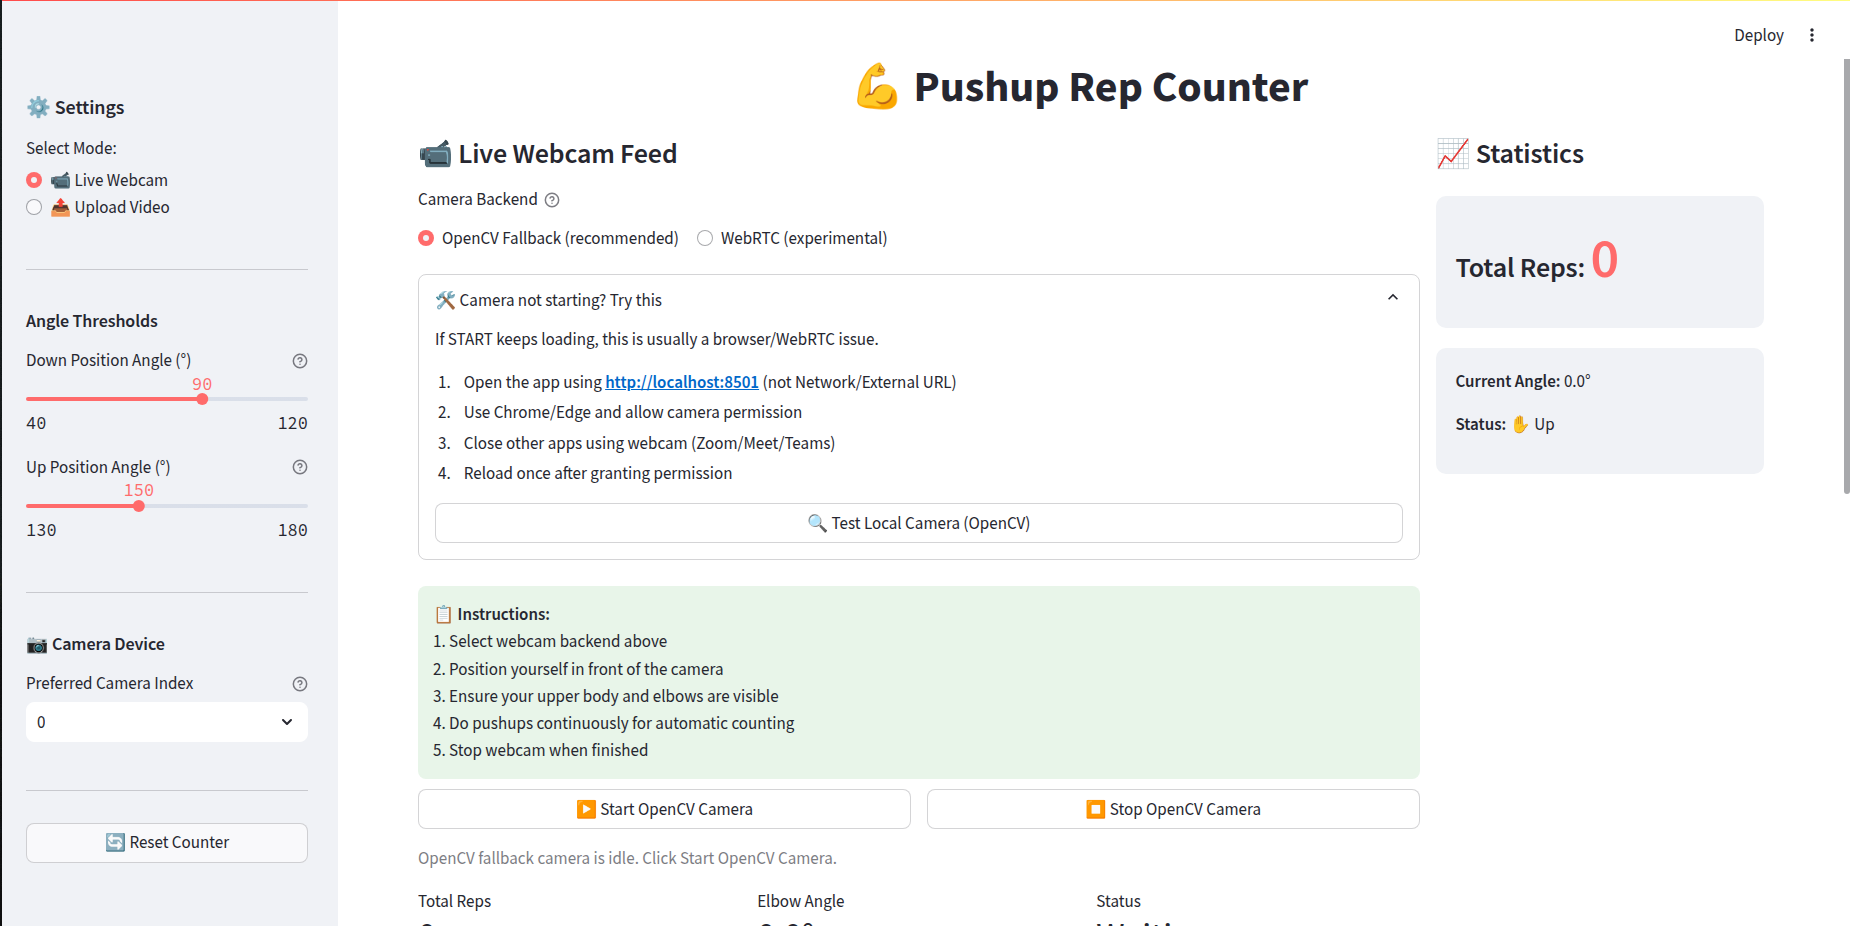
\includegraphics[width=0.85\textwidth]{Screenshots/ui_1.png}
    \caption{Main Interface: Live processing feed generating real-time predictions via OpenCV backend.}
\end{figure}

\begin{figure}[H]
    \centering
    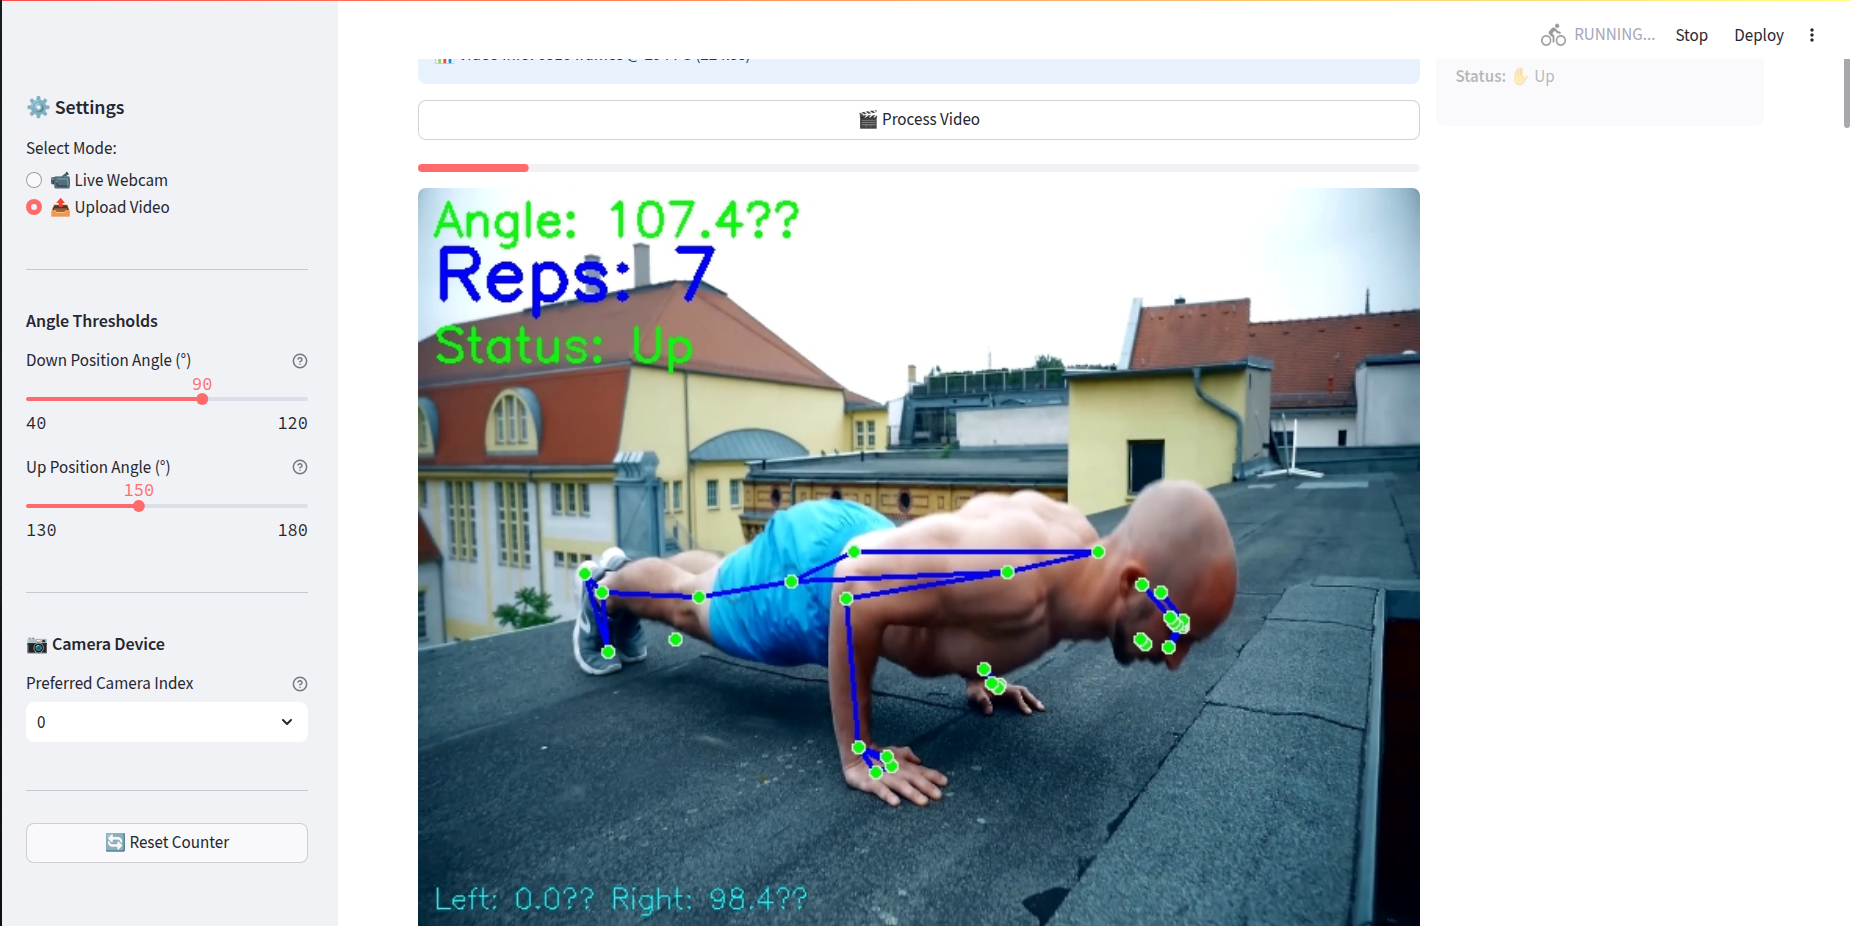
\includegraphics[width=0.85\textwidth]{Screenshots/ui_2.png}
    \caption{Video Upload Mode: Historical parsing of user-supplied Media, featuring live metric states (Pose: Down) and integrated skeleton rendering.}
\end{figure}

\begin{figure}[H]
    \centering
    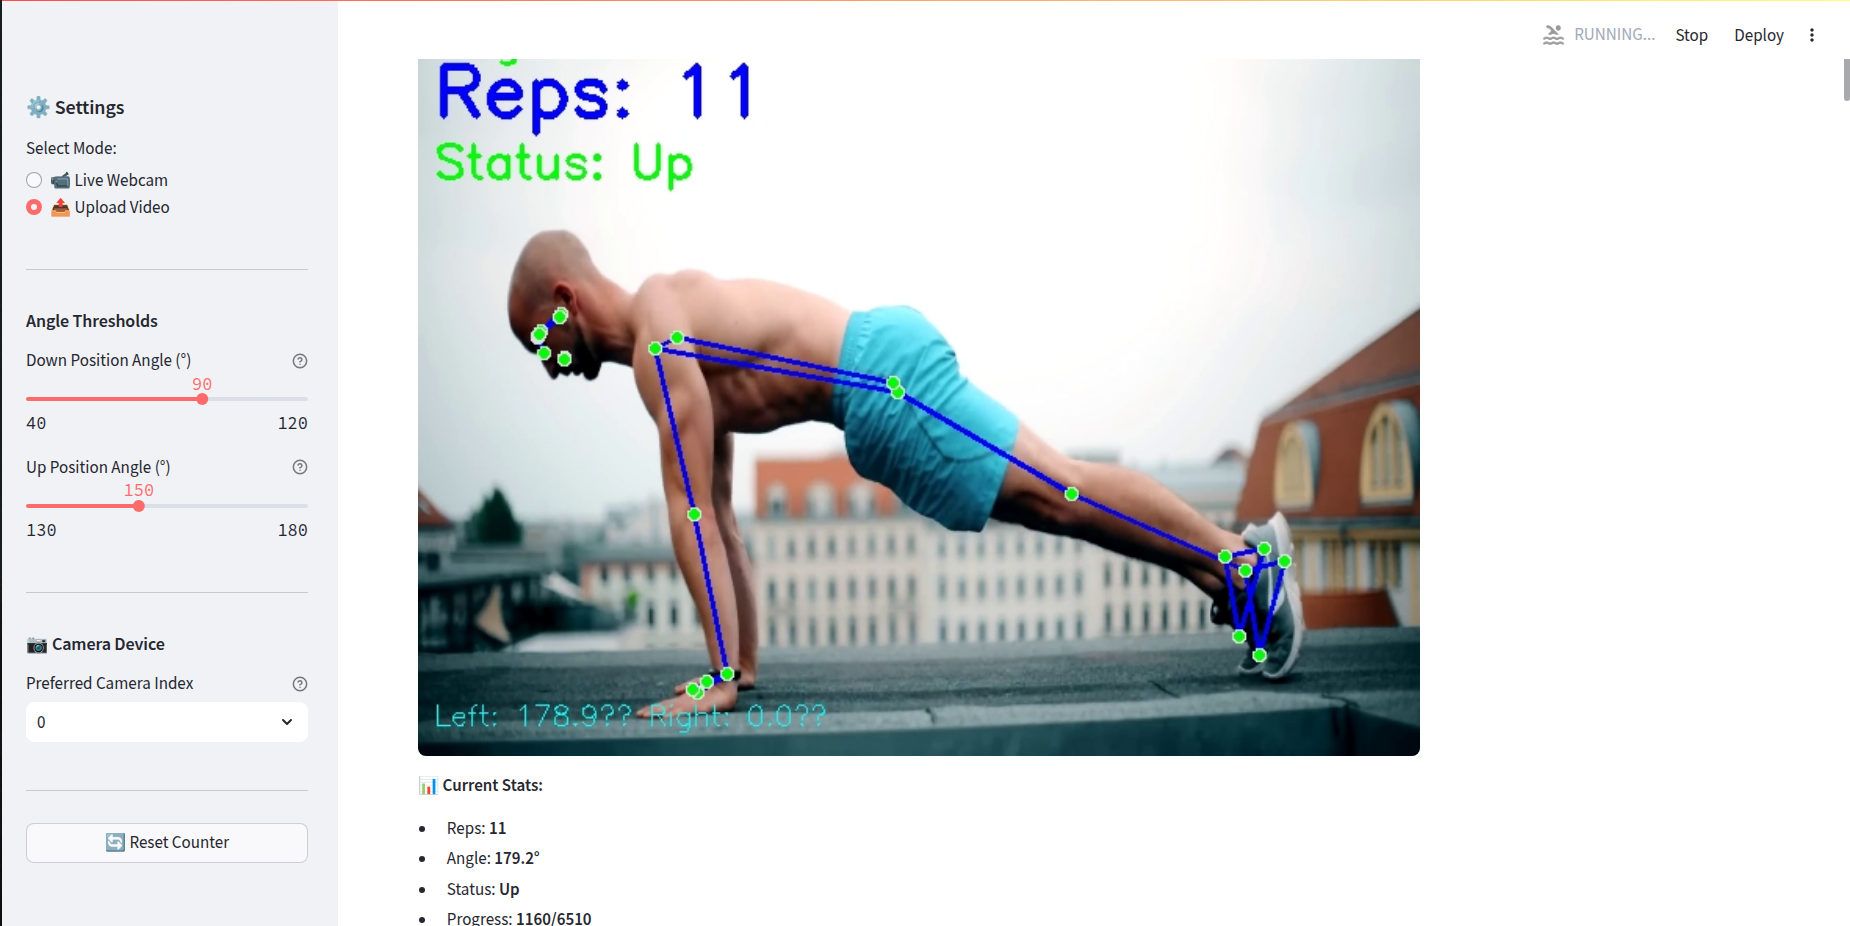
\includegraphics[width=0.85\textwidth]{Screenshots/ui_3.png}
    \caption{Metrics Dashboard: Interactive statistical analysis displaying frame-over-frame analytics post-processing.}
\end{figure}

\section{Conclusion}
The Pushup Rep Counter robustly meets all primary objectives, demonstrating a functional application of machine learning within personal fitness tracking. Relying upon geometric analysis of pose landmarks enabled the deployment of a zero-training, highly adaptable, and accessible platform.

\end{document}
